\documentclass[12pt,english,a4paper]{report}

\usepackage[utf8]{inputenc}          % Allows UTF-8 encoded characters in the .tex-file.
\usepackage{babel,csquotes,textcomp,duomasterforside} % Set LaTeX to structure the content following international academic standards.

\usepackage[toc,page]{appendix}

\usepackage{hyperref}
\usepackage{graphicx}
\usepackage{pdfpages}
\usepackage{listings}
\usepackage{wrapfig}
\usepackage{color,colortbl}
\usepackage{lettrine}
\usepackage[font={small,it}]{caption}
\usepackage{multirow}
\usepackage{tabularx}
\usepackage{footnote}
\usepackage{subfiles}
\usepackage{minted}
\usepackage{fancyvrb}
\usemintedstyle{friendly}

\newmintedfile[pythoncode]{python}{
fontsize=\scriptsize,
fontfamily=tt,
linenos=true,
numberblanklines=true,
numbersep=12pt,
numbersep=5pt,
gobble=0,
frame=leftline,
framerule=0.4pt,
framesep=2mm,
funcnamehighlighting=true,
tabsize=4,
obeytabs=false,
mathescape=false
samepage=false, %with this setting you can force the list to appear on the same page
showspaces=false,
showtabs =false,
texcl=false,
breaklines = true
}

\newmintedfile[ccode]{c}{
fontsize=\scriptsize,
fontfamily=tt,
linenos=true,
numberblanklines=true,
numbersep=12pt,
numbersep=5pt,
gobble=0,
frame=leftline,
framerule=0.4pt,
framesep=2mm,
funcnamehighlighting=true,
tabsize=4,
obeytabs=false,
mathescape=false
samepage=false, %with this setting you can force the list to appear on the same page
showspaces=false,
showtabs =false,
texcl=false,
breaklines = true
}

\newmintedfile[makecode]{make}{
fontsize=\scriptsize,
fontfamily=tt,
linenos=true,
numberblanklines=true,
numbersep=12pt,
numbersep=5pt,
gobble=0,
frame=leftline,
framerule=0.4pt,
framesep=2mm,
funcnamehighlighting=true,
tabsize=4,
obeytabs=false,
mathescape=false
samepage=false, %with this setting you can force the list to appear on the same page
showspaces=false,
showtabs =false,
texcl=false,
breaklines =true
}

% Making the whole paragraph biz possible
%\usepackage{titlesec}
%\setcounter{secnumdepth}{4}
%\titleformat{\paragraph}
%{\normalfont\normalsize\bfseries}{\theparagraph}{1em}{}
%\titlespacing*{\paragraph}
%{0pt}{3.25ex plus 1ex minus .2ex}{1.5ex plus .2ex}

% Adding the bib
\usepackage[
    backend=biber,
    style=numeric
]{biblatex}
\addbibresource{refs.bib}

\definecolor{mygreen}{rgb}{0,0.6,0}
\definecolor{mygray}{rgb}{0.5,0.5,0.5}
\definecolor{mymauve}{rgb}{0.58,0,0.82}
\definecolor{auxiliryc}{RGB}{70,240,161} %Green
\definecolor{ineffectivec}{RGB}{70,149,240} %purple
\definecolor{effectivec}{RGB}{115,70,240} % Blue

\graphicspath{{./graphics/}}

% Setting tty font?
%\lstset{ %
%  basicstyle=\ttfamily\small,     
%  backgroundcolor=\color{white},   % choose the background color
%  breaklines=true,                 % automatic line breaking only at whitespace
%  captionpos=b,                    % sets the caption-position to bottom
%  commentstyle=\color{mygreen},    % comment style
%  escapeinside={\%*}{*)},          % if you want to add LaTeX within your code
%  keywordstyle=\color{blue},       % keyword style
%  stringstyle=\color{mymauve},     % string literal style
%  showspaces=false,
%  showstringspaces=false,
%}

\lstset{language=C,
  basicstyle=\ttfamily\scriptsize,
  keywordstyle=\color{blue}\ttfamily,
  stringstyle=\color{red}\ttfamily,
  commentstyle=\color{green}\ttfamily,
  breaklines=true,
  showspaces=false,
  showstringspaces=false,
  numbers=left,                    % where to put the line-numbers; possible values are (none, left, right)
  numbersep=5pt,    
  frame=single,                 % how far the line-numbers are from the code
  numberstyle=\tiny\color{mygray}, % the style that is used for the line-numbers
  rulecolor=\color{black}         % if not set, the frame-color may be changed on line-breaks 
}

\title{GPS Spoofing}
\subtitle{A detection and mitigation system}
\author{Aril Schultzen}
\begin{document}
\duoforside[dept={Institutt for informatikk},
program={Informatikk: programmering og nettverk},
long]

\begin{abstract}
Abstract goes here.
\end{abstract}

\chapter*{Foreword}
Here goes foreword

% Hackish code to keep counters and white pages at bay
\thispagestyle{empty}
\setcounter{page}{0}
\tableofcontents
\thispagestyle{empty}
\setcounter{page}{0}
\thispagestyle{empty}
\setcounter{page}{0}
\clearpage
\setcounter{page}{1}

% Here goes all the chapters
% ==================================================

\subfile{intro}

% Chapter about the csac and it's connectivity?

\chapter{Method}

\section{Choice of hardware}
\begin{figure}\label{ibd}
  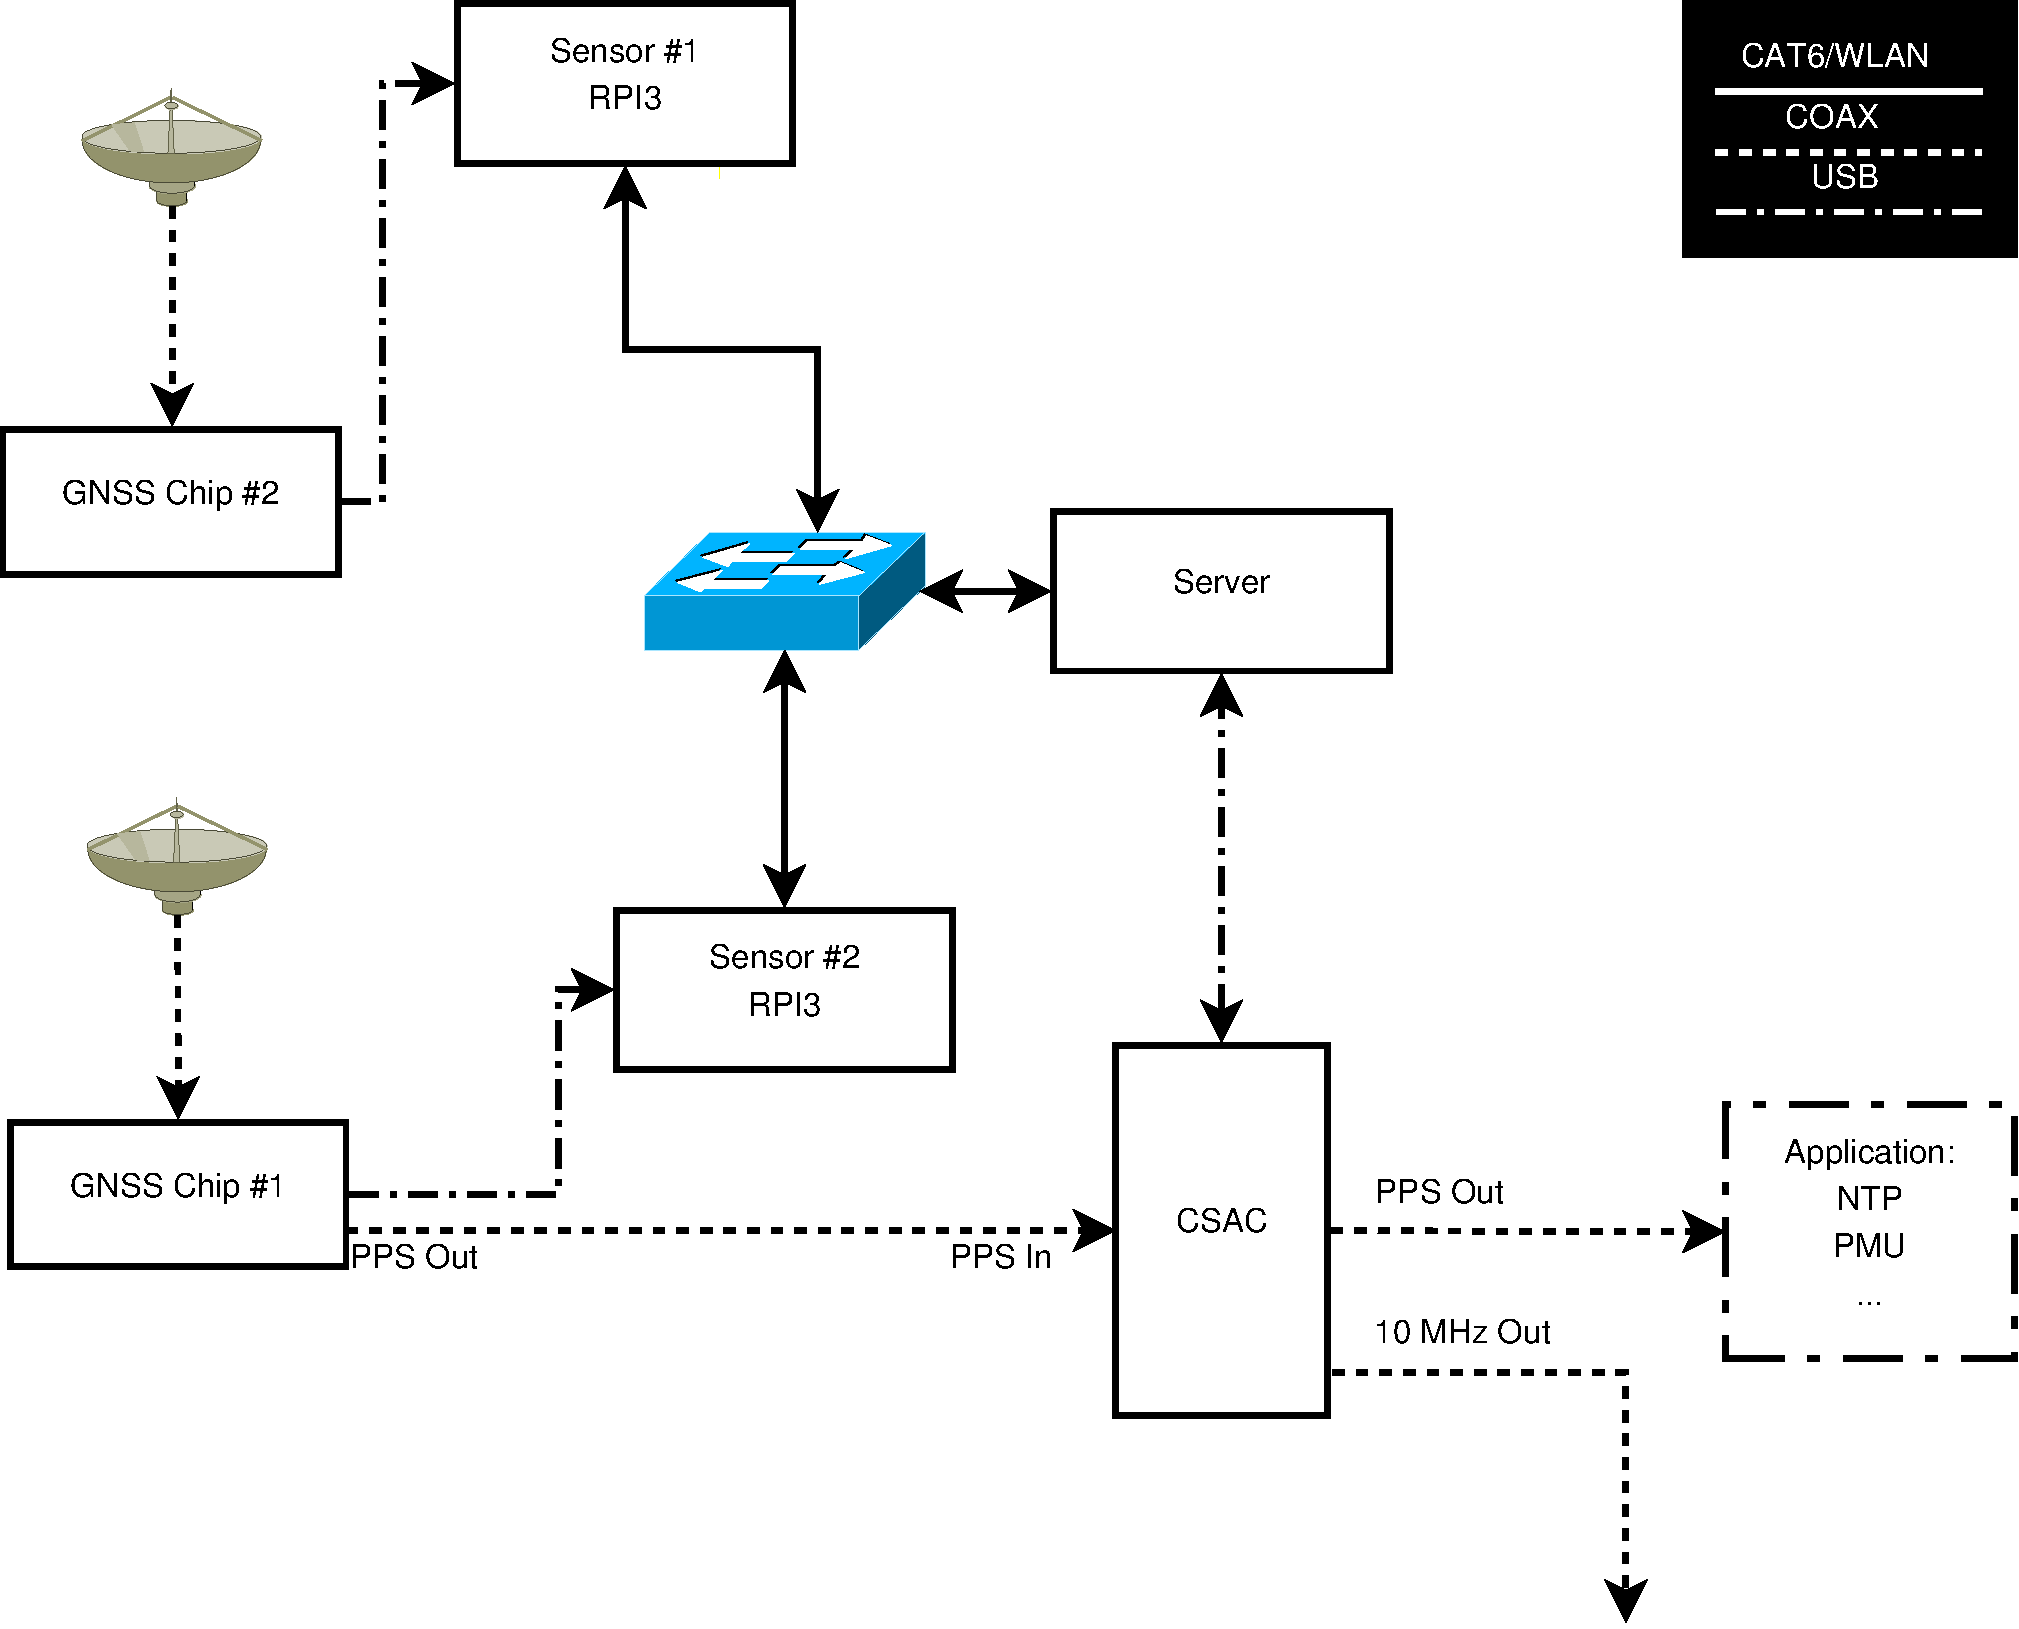
\includegraphics[angle=90, scale=0.5]{server_layout.pdf}
   \caption[CSAC SMACC implementation block diagram]{A block diagram showing the tested implementation}
\end{figure}

\subsection{Chip Scale Atomic Clock}
I propose to use the Symmetricom SA.45 as the CSAC. This is a CSAC measuring only 16cc with 1 pulse per second (PPS) output and 1 PPS input (for disciplining). The SA.45's strength is it's low power consumption (less than 120mW) and low price \cite{SADS}. The SA.45 also uses a built-in controller which can be communicated with over a RS-232 serial interface. The ability to communicate with the CSAC, issue commands and collect data, is paramount for the feasibility of our proposal. It's worth mentioning that any atomic clock such as Cesium standard or even a Rubidium standard could be used given that they have a means to communicate basic telemetry as used by the SMACC software.

\subsection{SMACC platform}
I propose to use the Raspberry Pi 3 Model B (RASPI3) in the role as the host running the SMACC software. The RASPI3 is an interesting piece of equipment with an impressive list of specifications. It is a single board computer with a 1.2GHz 64-bit quad-core ARMv8 CPU, 1 GB of RAM, built in 802.11n Wireless LAN and four USB ports (\cite{RASPI}) (just to mention some). As with the Symmetricom SA.45, the RASPI3 is very affordable and retailed at about 35 USD when this report was written. We also propose to use Raspbian (\cite{RASPBIAN}), a Debian derived flavor of Linux optimized for the Raspberry Pi as the operating system. 

\subsection{GNSS receiver}
I propose to use at least two GNSS receivers. Both of the receivers should simply collect data and feed it to the SMACC but one of the receivers should also double as a 1 PPS disciplining source for the CSAC. Considering that need for a stable 1 PPS source, I propose to use the u-blox M8T. This is a relativity affordable GNSS receiver with a temperature compensated crystal oscillator (TCXO), 3 concurrent GNSS reception and an external antenna (\cite{UBLOXM8T}). Currently, only strings of NMEA data is collected from the GNSS receiver. However in the future it might be beneficial to collect and process raw data from the receivers as well. Since most GNSS receivers today follow the NMEA standard (to some extent) and raw data currently isn't required, common and popular receivers like the u-blox NEO series should be more that sufficient to use in an implementation if this proposal.

\chapter{Software}
\section{Choice of programming language}
The SMACC software was originally planned to be written in Java since this was my most fluent programming language. Java is great language, it's object oriented, it has a garbage collector and a lot of useful libraries. As development started, it quickly became apparent that some parts of the code would be performance critical and that portability really wasn't that important anyway. The platform was already decided and there was no reason to believe that it would change in the near future. As we all know, premature optimization is the root of all evil. Being reluctant to commit a deadly programming sin, i decided to look at other languages. Since performance was a concern, Python was also quickly dismissed as an option. C++ would probably have been the best choice, but having never written anything in C before made it sound more exciting and like a nice opportunity to learn something new. During the planning phase of SMACC development, raspbian-2015-05-07 was the latest build. It came with GCC 4.6.3 which only had experimental support for C11(\cite{GCC11}). With C11 no longer considered an option, C99 was the obvious choice given it's attractive features like:
\begin{itemize}
  \item Variable-length arrays.
  \item Single line comments.
  \item snprintf() as standard (\cite{C_RATIONAL}).
\end{itemize}

\section{The Sensor Server/Client model}
Numerous approaches where considered when planning the implementation of the SMACC software (\ref{da}). The approach that was chosen is what I have named the "Sensor Server". The Sensor Server is based on the idea that a GNSS receiver and a computer can be viewed abstractly as a single device, a Sensor. The Sensor runs the sensor client software that communicates with the server. With this approach, a great number of GNSS receivers can be connected to the SMACC using existing infrastructure, communicating over IP. The Sensor Server implements the functionality that was planned for the SMACC to implement (\ref{op}) and then some more.

% Refer to protocol.h at the point when describing the ID process?
\section{The Sensor Client}
The sensor client software is a simple program written in C99 whose only task is to relay information read from the GNSS receivers. Summed up shortly:
\begin{itemize}
  \item The client software takes two parameters to start, the servers IP and port. If parameters are missing, the program exits.
  \begin{itemize}
    \item Example: \texttt{./sensor\_client -p 10000 -i 192.168.1.5}
  \end{itemize}
  \item Initializes and loads configuration from configuration file. The configuration file includes path to the GNSS receiver, the sensors ID number and a binary value for whether or not logging of NMEA should be done as well as path to 
  the log file. If the loading of the configuration file fails, default values are used instead:
  \begin{itemize}
    \item The ID number is chosen at random but within legal limits.
    \item Logging is disabled.
    \item Maximum of server connection attempts are set to 10.
    \item Path to GNSS receiver is set to \texttt{/dev/ttyACM0}. This should be the path to the receiver unless another similar device is connected to the computer and given it is a Raspberry Pi running Raspbian.
  \end{itemize}
  \item Establishes communication with GNSS receiver, exits if it fails.
  \item Attempts to establish communication with the server, retries for a configurable amount of times at 1 second intervals.
  \item Identifies the client for the server according to protocol.
  \item Reads from the GNSS receiver, scans for lines starting with either \texttt{\$GNRMC} or \texttt{\$GNGGA}. When both lines are found, the data is stored in a buffer.
  \item Sends the GNSS data to the server according to protocol.
  \item Repeats.
\end{itemize}

\section{The Sensor Server }

\subsection{Processes vs Threads}

\subsection{Shared memory}
Since the server needs to have access to all the data the clients transmit, it uses a shared memory model. Every process that forks out from the server is given access to this memory area. Even the processes themselves have access to each others memory. One might make the point that this voids the idea of processes, and one might be correct (see \ref{discussion}). The shared memory is created using the GNU library's Memory Mapped I/O (MMAP). Although typically used to map files to a region of memory, MMAP can also be used to create an anonymous map which is not connected to file but rather for sharing data between tasks without using files.

\begin{lstlisting}
client_list = mmap(NULL, 
                  (s_conf->max_clients * sizeof(struct client_table_entry)), 
                  PROT_READ | PROT_WRITE,
                  MAP_SHARED | MAP_ANONYMOUS,
                  -1, 0);
\end{lstlisting}
The example over shows how shared memory is allocated. The observant reader will notice that there memory is allocated for a finite number of clients. This is unfortunate but necessary: The fork operation creates a completely separate address space for the child process but the child still has a complete copy of parents memory segments. Since the child process is completely separated from the parent, any changes in the shared memory done by the parent will not be "reflected" in the child's memory. In other words, the entire shared memory \textit{has} to be initialized before any fork operations are done. Failing to do so will result in a segmentation fault once a process attempts to access the memory of a younger sibling. In this application however, we always know how many clients are going to connect. Even when in doubt, the maximum number of clients can be grossly overestimated and configured in order to make sure that there is room for more clients.

\subsection{Structs}
In the C programming language, a "struct" is a complex data type that defines a list of variables to be placed under the structs given name in a block of memory. This makes it possible for multiple variables to be accessed via a single pointer. Before delving deeper into the code base of the sensor server, some crucial and often used structs will be explained in this section.

\subsubsection{Client table entry}
The client\_table\_entry is what the name suggests, it's an entry in a list of clients. Every client connected to the server, no matter the purpose, has an entry in the client list. The entry in the list contains information about the client including but not limited to:
\begin{itemize}
  \item Process ID
  \item IP Address
  \item Client ID
  \item NMEA data (\ref{nmea_cont}).
  \item Filter data
\end{itemize}
Of all the pointers tossed about in the sensor server, this type is the most common one. 

\subsubsection{NMEA container}\label{nmea_cont}


\subsubsection{Components}
In the following sections, the different components that comprises the sensor server will be explained. 

\subsubsection{CSAC Communication}
  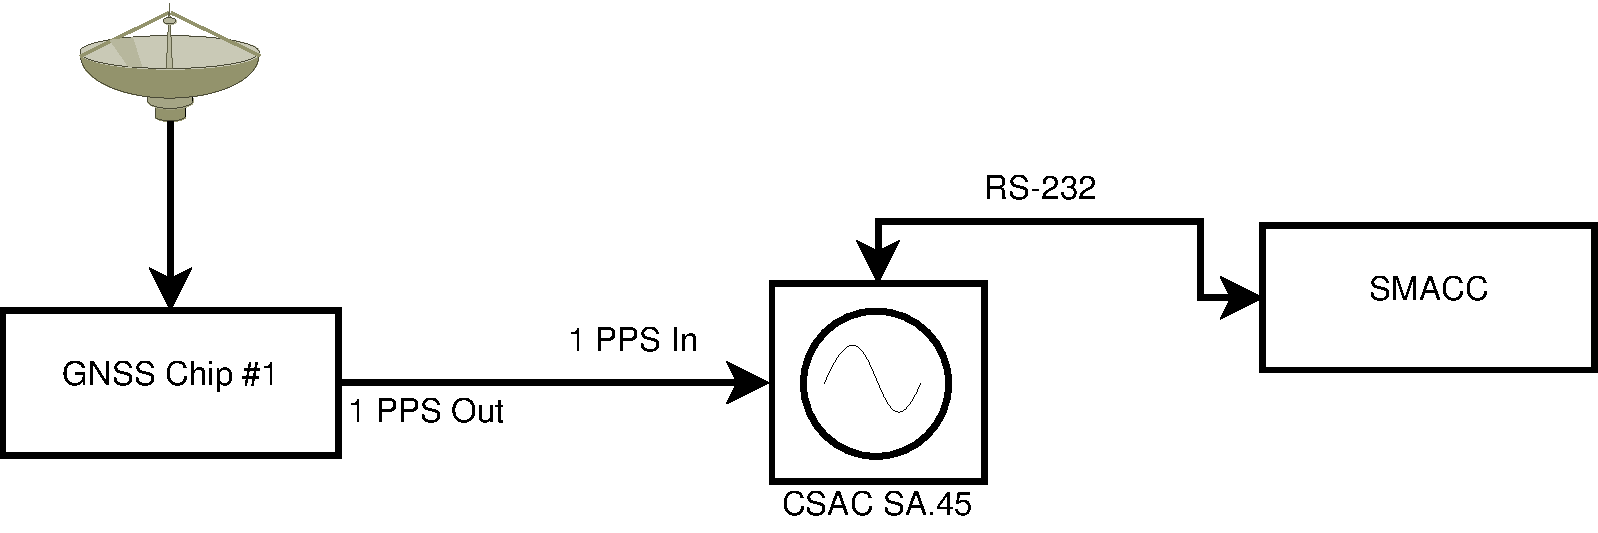
\includegraphics[width=1\textwidth]{csac_serial.pdf}
The SA.45 CSAC includes a serial interface that enables communication with a PC by using a COM port. As mentioned earlier, our approach relies heavily on the ability to communicate with the CSAC.
Information can be queried by sending commands to the CSAC. These commands are explained in table \ref{CSAC_COMMANDS}. 
\begin{table}[]
\centering
\caption{Commands for the SA.45 CSAC}
\label{CSAC_COMMANDS}
\begin{tabular}{|l|l|l|}
\hline
Shortcut          & Description                                        & Command                       \\ \hline
6                 & Return telemetry headers as comma-delimited string & !6{[}CRLF{]}                  \\ \hline
\textasciicircum  & Return telemetry as comma-delimited string         & !\textasciicircum  {[}CRLF{]} \\ \hline
F                 & Adjust frequency                                   & !F?{[}CRLF{]}                 \\ \hline
M                 & Set operating mode register bits                   & !M?{[}CRLF{]}                 \\ \hline
S                 & Sync CSAC 1 PPS to external 1 PPS                  & !S{[}CRLF{]}                  \\ \hline
D                 & Set 1 PPS disciplining time constant               & !D?{[}CRLF{]}                 \\ \hline
U                 & Set ultra-low power mode parameters                & !U?{[}CRLF{]}                 \\ \hline
T                 & Set/report time-of-day                             & !T?{[}CRLF{]}                 \\ \hline
\end{tabular}
\caption*{Source: \cite{CSAC_USERGUIDE}}
\end{table}

\section{Detection algorithms: Filters}
\subsection{Data acquisition}\label{data_aquisition}
In order to create an accurate clock-model of the CSAC, it was necessary to log data from it while it was running in a disciplined mode. In the disciplined mode, the CSAC will correct it's frequency based on either a 1 PPS (Pulse per second) signal or a 10 MHz signal. A similar approach was used in order to collect GPS data. Data from two u-blox M8T was gathered over the same time period as the data gathered from the CSAC. By gathering the data over the same period, it was possible to detect any correlation between the time solved by the GPS receivers and any frequency adjustments done by the CSAC. It also provided valuable data that could be used to tune the spoofing detection algorithms in the CSAC SMACC. The data gathering was done by simple Python scripts (\ref{CL} and \ref{GL}) running on a computer connected to the receivers and the CSAC (\ref{CLS})

\subsubsection{Clock Model}
Write about clock model

\subsubsection{Naive MIN-MAX filter}
The MIN-MAX filter is one of the least sophisticated filters implemented. Data is gathered over a pre-determined "warm-up" period and the server compares the lowest and highest values of this data with current data. If the values are either higher or lower than the collected data, the data is considered abnormal. 

\subsubsection{Probability filter}
The "probability filter" is implemented by using collected data to create a model of expected data. The current data is then compared in order to evaluate whether or not it is abnormal. 

\chapter{Testing}

\section{Software performance}
How was the performance of the server? Slow? Buggy?

\section{Preliminary test}
Write about the simple test where I moved the antennas about.

\section{Spoof test}
\subsection{Challenges}
What if their clocks sucks?

\subsection{The test}
Write about the test

\chapter{Results and discussion}\label{discussion}

\section{Different approaches}\label{da}
When planning on how to execute our proposal, these where among the ideas that came up. 

\subsubsection{Single computer, many GNSS receivers}
A single computer is used to run the SMACC software. The SMACC does not include a socket server, but the receivers used to collect data are all connected to to the computer through whatever USB ports available or made available by the use of USB hubs. With this approach, you are not dependent on a network, but it limits the number of GNSS receivers you could connect as the USB specification limits the number possible endpoints to an absolute 127(\cite[pp. 3]{USBTC}) because of addressing. This does not mean that 127 devices can be connected, a single device might use more than one endpoint. It's also worth mentioning that a USB hub might "reserve" multiple endpoints. Depending on the GNSS receivers and how they are made, this number might be reduced even further by the power usage of the connected devices. Depending on how far each GNSS receiver is distanced from the SMACC, a signal amplifier might be necessary to compensate for the signal attenuation. In some cases where a network is absent, this might be only option.

\subsubsection{Store in database and analyze}
With this approach, the idea of a GNSS receiver and RASPI as a single "sensor" unit is the same as with Client-server approach. The difference is that it with this approach, each sensor stores the collected data in a database. The SMACC software monitors the clock directly as with the Client-server approach, but the data in the database is routinely queried and analyzed. The strength with this approach is that data is easily stored, shared and maintained by a single entity. The complexity of the client software would be the same as with Client-server approach, but the SMACC software could be implemented with less complexity as no Client-server architecture or shared memory schemes would be necessary. During planning, this approach seemed promising but was rejected because it was thought that it might not be time-sensitive enough. It was also some doubt concerning whether or not the ability to store data to a database actually was important. Once the different filters and algorithms was in place, it turned that the database functionality would have been nice, but not of any real importance for the SMACC to perform it's tasks, and would have been overkill anyway.

\chapter{Conclusion}
You should have done things different.

\subfile{appendix}

%===================================================

\newpage
\printbibliography[title={Complete Bibliography},heading=bibintoc]

\end{document}                    